\section{Results} \label{section:results}

In order to reflect on how well our models have been trained on different datasets, we report the perplexity for each experiment along with the training steps (from nmt) or epochs (from fairseq). During the training, we stored the model checkpoints of step or epoch which led to the best\footnote{Depending on the support of the frameworks, we stored the one with best validation BLEU in nmt and the one with best validation loss in fairseq.} performance on the validation set in a model checkpoint file which is later used to perform decoding on the test set and report the BLEU scores. This section describes the statistical results of the 40 experiments, while their analysis and implications are discussed in Section \ref{section:discussion}.

\subsection{Perplexities} \label{subsection:perplexity}

Figure \ref{fig:monu600 ppls} shows the graphs of the training and validation perplexity during the training of each model on the MonumentNSpM dataset. Compared to other two monument splits, this dataset has the largest number of training examples, where a full epoch for the fairseq is approximately equivalent to 120 steps for the nmt. After a sufficient number of iterations, all of the models are able to achieve a relatively low perplexity (close to 1) on the training set which means a nearly perfect fitting. On the validation set, all of the models converged at a perplexity between 1 and 1.25, although slight overfittings are observed on two attention-equipped NSpM models as shown in Figure \ref{fig:monu600 nsmbah ppl} and \ref{fig:monu600 nsmluo ppl}. In Figure \ref{fig:monu600 transformer ppl} we noticed an unusual phenomenon that the validation perplexity is lower than the training in early epochs.

Figure \ref{fig:monu1 ppls} shows the perplexity graphs on the Monument80 dataset. For this dataset, around 100 steps in the nmt are equivalent to an epoch in the fairseq. The trend of each model is similar with the MonumentNSpM dataset. Given the fact that this dataset contains more validation examples and less training examples than the MonumentNSpM dataset, the validation perplexities are mostly higher but still within the range 1 to 1.5. Slight overfittings are continued to be observed in Figure \ref{fig:monu1 nsm-bah ppl}, \ref{fig:monu1 nsm-luo ppl}, \ref{fig:monu1 gnmt4 ppl}, and \ref{fig:monu1 gnmt8 ppl}.
% Monument NSpM ppls
\begin{figure}[H]
\centering
\begin{subfigure}{0.45\textwidth}
\includegraphics[width=\textwidth]{../results/monument_600/run1/neural_sparql_machine/ppls.png} 
\caption{NSpM}
\label{fig:monu600 nsm ppl}
\end{subfigure}
\hfill
\begin{subfigure}{0.45\textwidth}
\includegraphics[width=\textwidth]{../results/monument_600/run1/neural_sparql_machine_bahdanau_attention/ppls.png}
\caption{NSpM+Att1}
\label{fig:monu600 nsmbah ppl}
\end{subfigure}
\hfill
\begin{subfigure}{0.45\textwidth}
\includegraphics[width=\textwidth]{../results/monument_600/run1/neural_sparql_machine_luong_attention/ppls.png} 
\caption{NSpM+Att2}
\label{fig:monu600 nsmluo ppl}
\end{subfigure}
\hfill
\begin{subfigure}{0.45\textwidth}
\includegraphics[width=\textwidth]{../results/monument_600/run1/lstm_luong_wmt_en_de/ppls.png}
\caption{LSTM\_Luong}
\label{fig:monu600 lstm ppl}
\end{subfigure}
\hfill
\begin{subfigure}{0.45\textwidth}
\includegraphics[width=\textwidth]{../results/monument_600/run1/wmt16_gnmt_4_layer/ppls.png} 
\caption{GNMT-4}
\label{fig:monu600 gnmt4 ppl}
\end{subfigure}
\hfill
\begin{subfigure}{0.45\textwidth}
\includegraphics[width=\textwidth]{../results/monument_600/run1/wmt16_gnmt_8_layer/ppls.png}
\caption{GNMT-8}
\label{fig:monu600 gnmt8 ppl}
\end{subfigure}
\hfill
\begin{subfigure}{0.45\textwidth}
\includegraphics[width=\textwidth]{../results/monument_600/run2/fconv_wmt_en_de/ppls.png} 
\caption{ConvS2S}
\label{fig:monu600 convs2s ppl}
\end{subfigure}
\hfill
\begin{subfigure}{0.45\textwidth}
\includegraphics[width=\textwidth]{../results/monument_600/run1/transformer_iwslt_de_en/ppls.png}
\caption{Transformer}
\label{fig:monu600 transformer ppl}
\end{subfigure}
\hfill
\caption{Plots of perplexity on the training and validation set of MonumentNSpM for each model}
\label{fig:monu600 ppls}
\end{figure}

% Monument80 ppls
\begin{figure}[H]
\centering
\begin{subfigure}{0.45\textwidth}
\includegraphics[width=\textwidth]{../results/monument2_1/run1/neural_sparql_machine/ppls.png} 
\caption{NSpM}
\label{fig:monu1 nsm ppl}
\end{subfigure}
\hfill
\begin{subfigure}{0.45\textwidth}
\includegraphics[width=\textwidth]{../results/monument2_1/run1/neural_sparql_machine_bahdanau_attention/ppls.png}
\caption{NSpM+Att1}
\label{fig:monu1 nsm-bah ppl}
\end{subfigure}
\hfill
\begin{subfigure}{0.45\textwidth}
\includegraphics[width=\textwidth]{../results/monument2_1/run1/neural_sparql_machine_luong_attention/ppls.png} 
\caption{NSpM+Att2}
\label{fig:monu1 nsm-luo ppl}
\end{subfigure}
\hfill
\begin{subfigure}{0.45\textwidth}
\includegraphics[width=\textwidth]{../results/monument2_1/run1/lstm_luong_wmt_en_de/ppls.png}
\caption{LSTM\_Luong}
\label{fig:monu1 lstm ppl}
\end{subfigure}
\hfill
\begin{subfigure}{0.45\textwidth}
\includegraphics[width=\textwidth]{../results/monument2_1/run1/wmt16_gnmt_4_layer/ppls.png} 
\caption{GNMT-4}
\label{fig:monu1 gnmt4 ppl}
\end{subfigure}
\hfill
\begin{subfigure}{0.45\textwidth}
\includegraphics[width=\textwidth]{../results/monument2_1/run1/wmt16_gnmt_8_layer/ppls.png}
\caption{GNMT-8}
\label{fig:monu1 gnmt8 ppl}
\end{subfigure}
\hfill
\begin{subfigure}{0.45\textwidth}
\includegraphics[width=\textwidth]{../results/monument2_1/run2/fconv_wmt_en_de/ppls.png} 
\caption{ConvS2S}
\label{fig:monu1 convs2s ppl}
\end{subfigure}
\hfill
\begin{subfigure}{0.45\textwidth}
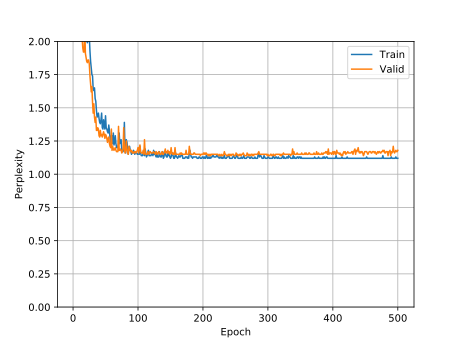
\includegraphics[width=\textwidth]{../results/monument2_1/run1/transformer_iwslt_de_en/ppls.png}
\caption{Transformer}
\label{fig:monu1 transformer ppl}
\end{subfigure}
\hfill
\caption{Plots of perplexity on the training and validation set of Monument80 for each model}
\label{fig:monu1 ppls}
\end{figure}

% Monument50 ppls
\begin{figure}[H]
\centering
\begin{subfigure}{0.45\textwidth}
\includegraphics[width=\textwidth]{../results/monument2_2/run1/neural_sparql_machine/ppls.png} 
\caption{NSpM}
\label{fig:monu2 nsm ppl}
\end{subfigure}
\hfill
\begin{subfigure}{0.45\textwidth}
\includegraphics[width=\textwidth]{../results/monument2_2/run1/neural_sparql_machine_bahdanau_attention/ppls.png}
\caption{NSpM+Att1}
\label{fig:monu2 nsm-bah ppl}
\end{subfigure}
\hfill
\begin{subfigure}{0.45\textwidth}
\includegraphics[width=\textwidth]{../results/monument2_2/run1/neural_sparql_machine_luong_attention/ppls.png} 
\caption{NSpM+Att2}
\label{fig:monu2 nsm-luo ppl}
\end{subfigure}
\hfill
\begin{subfigure}{0.45\textwidth}
\includegraphics[width=\textwidth]{../results/monument2_2/run1/lstm_luong_wmt_en_de/ppls.png}
\caption{LSTM\_Luong}
\label{fig:monu2 lstm ppl}
\end{subfigure}
\hfill
\begin{subfigure}{0.45\textwidth}
\includegraphics[width=\textwidth]{../results/monument2_2/run1/wmt16_gnmt_4_layer/ppls.png} 
\caption{GNMT-4}
\label{fig:monu2 gnmt4 ppl}
\end{subfigure}
\hfill
\begin{subfigure}{0.45\textwidth}
\includegraphics[width=\textwidth]{../results/monument2_2/run1/wmt16_gnmt_8_layer/ppls.png}
\caption{GNMT-8}
\label{fig:monu2 gnmt8 ppl}
\end{subfigure}
\hfill
\begin{subfigure}{0.45\textwidth}
\includegraphics[width=\textwidth]{../results/monument2_2/run2/fconv_wmt_en_de/ppls.png} 
\caption{ConvS2S}
\label{fig:monu2 convs2s ppl}
\end{subfigure}
\hfill
\begin{subfigure}{0.45\textwidth}
\includegraphics[width=\textwidth]{../results/monument2_2/run1/transformer_iwslt_de_en/ppls.png}
\caption{Transformer}
\label{fig:monu2 transformer ppl}
\end{subfigure}
\hfill
\caption{Plots of perplexity on the training and validation set of Monument50 for each model}
\label{fig:monu2 ppls}
\end{figure}

% LC-QUAD ppls
\begin{figure}[H]
\centering
\begin{subfigure}{0.45\textwidth}
\includegraphics[width=\textwidth]{../results/lc-quad1/run1/neural_sparql_machine/ppls.png} 
\caption{NSpM}
\label{fig:lcquad nsm ppl}
\end{subfigure}
\hfill
\begin{subfigure}{0.45\textwidth}
\includegraphics[width=\textwidth]{../results/lc-quad1/run1/neural_sparql_machine_bahdanau_attention/ppls.png}
\caption{NSpM+Att1}
\label{fig:lcquad nsm-bah ppl}
\end{subfigure}
\hfill
\begin{subfigure}{0.45\textwidth}
\includegraphics[width=\textwidth]{../results/lc-quad1/run1/neural_sparql_machine_luong_attention/ppls.png} 
\caption{NSpM+Att2}
\label{fig:lcquad nsm-luo ppl}
\end{subfigure}
\hfill
\begin{subfigure}{0.45\textwidth}
\includegraphics[width=\textwidth]{../results/lc-quad1/run1/lstm_luong_wmt_en_de/ppls.png}
\caption{LSTM\_Luong}
\label{fig:lcquad lstm ppl}
\end{subfigure}
\hfill
\begin{subfigure}{0.45\textwidth}
\includegraphics[width=\textwidth]{../results/lc-quad1/run1/wmt16_gnmt_4_layer/ppls.png} 
\caption{GNMT-4}
\label{fig:lcquad gnmt4 ppl}
\end{subfigure}
\hfill
\begin{subfigure}{0.45\textwidth}
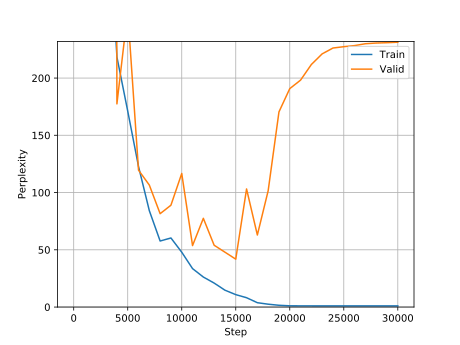
\includegraphics[width=\textwidth]{../results/lc-quad1/run1/wmt16_gnmt_8_layer/ppls.png}
\caption{GNMT-8}
\label{fig:lcquad gnmt8 ppl}
\end{subfigure}
\hfill
\begin{subfigure}{0.45\textwidth}
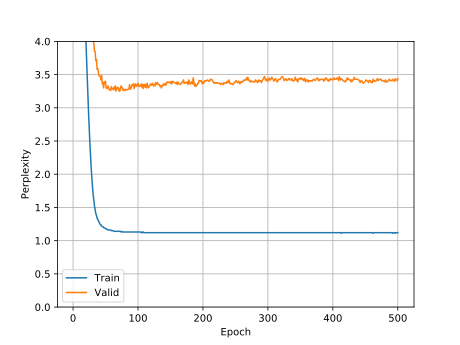
\includegraphics[width=\textwidth]{../results/lc-quad1/run2/fconv_wmt_en_de/ppls.png} 
\caption{ConvS2S}
\label{fig:lcquad convs2s ppl}
\end{subfigure}
\hfill
\begin{subfigure}{0.45\textwidth}
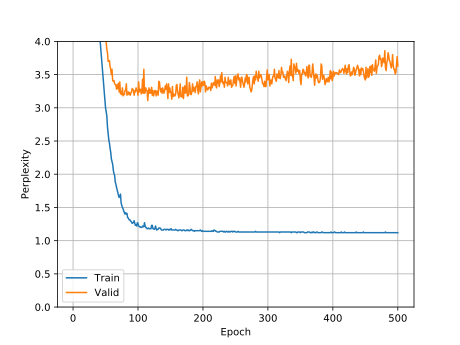
\includegraphics[width=\textwidth]{../results/lc-quad1/run1/transformer_iwslt_de_en/ppls.png}
\caption{Transformer}
\label{fig:lcquad transformer ppl}
\end{subfigure}
\hfill
\caption{Plots of perplexity on the training and validation set of LC-QUAD for each model}
\label{fig:lcquad ppls}
\end{figure}

%DBNQA ppls
\begin{figure}[H]
\centering
\begin{subfigure}{0.45\textwidth}
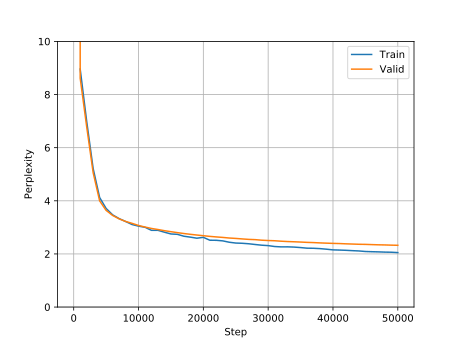
\includegraphics[width=\textwidth]{../results/dbnqa1/run1/neural_sparql_machine/ppls.png} 
\caption{NSpM}
\label{fig:dbnqa nsm ppl}
\end{subfigure}
\hfill
\begin{subfigure}{0.45\textwidth}
\includegraphics[width=\textwidth]{../results/dbnqa1/run1/neural_sparql_machine_bahdanau_attention/ppls.png}
\caption{NSpM+Att1}
\label{fig:dbnqa nsm-bah ppl}
\end{subfigure}
\hfill
\begin{subfigure}{0.45\textwidth}
\includegraphics[width=\textwidth]{../results/dbnqa1/run1/neural_sparql_machine_luong_attention/ppls.png} 
\caption{NSpM+Att2}
\label{fig:dbnqa nsm-luo ppl}
\end{subfigure}
\hfill
\begin{subfigure}{0.45\textwidth}
\includegraphics[width=\textwidth]{../results/dbnqa1/run1/lstm_luong_wmt_en_de/ppls.png}
\caption{LSTM\_Luong}
\label{fig:dbnqa lstm ppl}
\end{subfigure}
\hfill
\begin{subfigure}{0.45\textwidth}
\includegraphics[width=\textwidth]{../results/dbnqa1/run1/wmt16_gnmt_4_layer/ppls.png} 
\caption{GNMT-4}
\label{fig:dbnqa gnmt4 ppl}
\end{subfigure}
\hfill
\begin{subfigure}{0.45\textwidth}
\includegraphics[width=\textwidth]{../results/dbnqa1/run1/wmt16_gnmt_8_layer/ppls.png}
\caption{GNMT-8}
\label{fig:dbnqa gnmt8 ppl}
\end{subfigure}
\hfill
\begin{subfigure}{0.45\textwidth}
\includegraphics[width=\textwidth]{../results/dbnqa1/run1/fconv_wmt_en_de/ppls.png} 
\caption{ConvS2S}
\label{fig:dbnqa convs2s ppl}
\end{subfigure}
\hfill
\begin{subfigure}{0.45\textwidth}
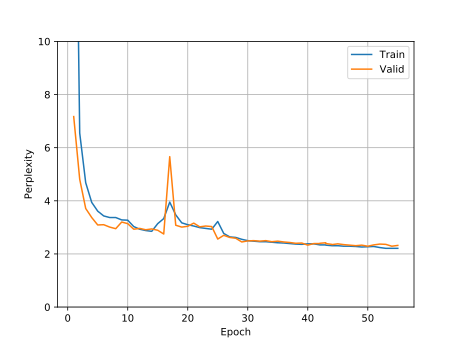
\includegraphics[width=\textwidth]{../results/dbnqa1/run1/transformer_iwslt_de_en/ppls.png}
\caption{Transformer}
\label{fig:dbnqa transformer ppl}
\end{subfigure}
\hfill
\caption{Plots of perplexity on the training and validation set of DBNQA for each model}
\label{fig:dbnqa ppls}
\end{figure}
Next, in order to assess the complexity of the monument dataset, we experimented on the Monument50 by further reducing the number of training examples but keeping the same size of the validation set. Here, one epoch is equivalent to 60 steps. The perplexity graphs are shown in Figure \ref{fig:monu2 ppls}. Although the training size is nearly half cut, it appears that the performance on the validation set are not much affected, especially for LSTM\_Luong, ConvS2S, and Transformer which are all implemented in the fairseq. This phenomenon is also reflected on BLEU scores in Table \ref{table:monu50 bleu} and Table \ref{table:monu80 bleu}.  

In the perplexity graphs on the LC-QUAD dataset shown in Figure \ref{fig:lcquad ppls}, we observed a noticeable difference between five models (Figure \ref{fig:lcquad nsm ppl}, \ref{fig:lcquad nsm-bah ppl}, \ref{fig:lcquad nsm-luo ppl}, \ref{fig:lcquad gnmt4 ppl} and \ref{fig:lcquad gnmt8 ppl} have shown serious overfitting at the time of convergence) implemented by the nmt and three models (Figure \ref{fig:lcquad lstm ppl}, \ref{fig:lcquad convs2s ppl} and \ref{fig:lcquad transformer ppl}) implemented by the fairseq. LC-QUAD is much smaller but more complicated compared to other datasets. It only takes 34 steps to finish training an epoch inside the nmt framework. Most of the models have difficulty of providing low perplexity on the validation set, among which GNMT-8 performed the worst and ConvS2S the best. 

Finally, Figure \ref{fig:dbnqa ppls} demonstrates the perplexities on the DBNQA dataset. Across all of the models, no evident overfitting is spotted. In a batch size of 128, an epoch of DBNQA takes nearly 5,600 training steps. Due to the large size of DBNQA, some models like NSpM and GNMT-8 have shown rather slow or incomplete convergence since the maximum training steps for them (50k and 30k) are just equivalent to a small number (10 and 6) of epochs. Nevertheless, all of the models have reached a perplexity of at least 2 on the validation set, where NSpM+Att1, NSpM+Att2, and ConvS2S have achieved lower than 2 as shown in Figure \ref{fig:dbnqa nsm-bah ppl}, \ref{fig:dbnqa nsm-luo ppl}, and \ref{fig:dbnqa convs2s ppl}.


\subsection{BLEU Scores}

The BLEU scores of the best checkpoint from each model are stated in Table \ref{table:monu600 bleu}-\ref{table:dbnqa bleu}. In each table, we primarily listed the BLEU scores on the validation and test set as well as the corresponding index of step or epoch of the selected model checkpoint. In order to refer to the state of the checkpoint at that step or epoch, we also reported the perplexities measured on the training and validation set.

\begin{table}[H]
\centering
\caption{BLEU scores and other information of the best checkpoint from each model on MonumentNSpM dataset}
\label{table:monu600 bleu}
\begin{tabular}{c|c|c|c|c|c}
Models & Train ppl & Valid ppl & \textbf{Valid BLEU} & \textbf{Test BLEU} & Step / Epoch \\
\hline
NSpM & 1.00 & 1.09 & 80.43 & 80.28 & Step 29k \\
NSpM+Att1 & 1.01 & 1.16 & 80.36 & 80.58 & Step 14k \\
NSpM+Att2 & 1.01 & 1.14 & 80.88 & 80.03 & Step 9k \\
GNMT-4 & 1.03 & 1.11 & 80.12 & 79.53 & Step 11k \\
GNMT-8 & 1.04 & 1.15 & 79.30 & 79.07 & Step 10k \\
LSTM\_Luong & 1.11 & 1.19 & 92.39 & 91.67 & Epoch 500 \\
ConvS2S & 1.11 & 1.14 & \textbf{98.35} & \textbf{97.12} & Epoch 500 \\
Transformer & 1.13 & 1.09 & 95.25 & 95.31 & Epoch 138 \\
\end{tabular}
\end{table}

In Table \ref{table:monu600 bleu}-\ref{table:monu50 bleu}, we reported the BLEU scores on three splits of the monument dataset. In all of these experiments, ConvS2S performed the best. It is also the case that LSTM\_Luong, ConvS2S, and Transformer outperformed other models by a large margin (about 10-15 BLEUs), most evident on the MonumentNSpM experiments.

\begin{table}[H]
\centering
\caption{BLEU scores and other information of the best checkpoint from each model on Monument80 dataset}
\label{table:monu80 bleu}
\begin{tabular}{c|c|c|c|c|c}
Models & Train ppl & Valid ppl & \textbf{Valid BLEU} & \textbf{Test BLEU} & Step / Epoch \\
\hline
NSpM & 1.00 & 1.21 & 87.55 & 87.03 & Step 44k \\
NSpM+Att1 & 1.00 & 1.44 & 87.82 & 87.34 & Step 44k \\
NSpM+Att2 & 1.00 & 1.44 & 87.99 & 87.37 & Step 34k \\
GNMT-4 & 1.00 & 1.31 & 85.94 & 85.39 & Step 30k \\
GNMT-8 & 1.01 & 1.32 & 84.94 & 84.14 & Step 30k \\
LSTM\_Luong & 1.11 & 1.24 & 96.35 & 96.12 & Epoch 200 \\
ConvS2S & 1.11 & 1.19 & \textbf{96.74} & \textbf{96.47} & Epoch 500 \\
Transformer & 1.12 & 1.14 & 95.16 & 94.87 & Epoch 267 \\
\end{tabular}
\end{table}

\begin{table}[H]
\centering
\caption{BLEU scores and other information of the best checkpoint from each model on Monument50 dataset}
\label{table:monu50 bleu}
\begin{tabular}{c|c|c|c|c|c}
Models & Train ppl & Valid ppl & \textbf{Valid BLEU} & \textbf{Test BLEU} & Step / Epoch \\
\hline
NSpM & 1.00 & 1.29 & 85.19 & 85.54 & Step 50k \\
NSpM+Att1 & 1.00 & 1.60 & 85.98 & 86.17 & Step 50k \\
NSpM+Att2 & 1.00 & 1.62 & 86.60 & 86.52 & Step 50k \\
GNMT-4 & 1.00 & 1.41 & 82.92 & 83.01 & Step 30k \\
GNMT-8 & 1.00 & 1.59 & 80.35 & 80.76 & Step 30k \\
LSTM\_Luong & 1.11 & 1.26 & 94.05 & 94.75 & Epoch 500 \\
ConvS2S & 1.11 & 1.20 & \textbf{96.44} & \textbf{96.62} & Epoch 500 \\
Transformer & 1.14 & 1.17 & 93.80 & 93.92 & Epoch 108 \\
\end{tabular}
\end{table}

Table \ref{table:lc-quad bleu} shows the performance of each model on the LC-QUAD dataset. The models all achieved relatively lower BLEU scores on this dataset as well as higher perplexities compared to other datasets. Another thing to notice is that the best checkpoints selected here are all from the middle stages of the training, which correlates with the potential overfittings exhibited in Figure \ref{fig:lcquad ppls}.

\begin{table}[H]
\centering
\caption{BLEU scores and other information of the best checkpoint from each model on LC-QUAD dataset}
\label{table:lc-quad bleu}
\begin{tabular}{c|c|c|c|c|c}
Models & Train ppl & Valid ppl & \textbf{Valid BLEU} & \textbf{Test BLEU} & Step / Epoch \\
\hline
NSpM & 1.00 & 16.46 & 43.91 & 43.50 & Step 20k \\
NSpM+Att1 & 1.00 & 56.23 & 52.68 & 50.13 & Step 40k \\
NSpM+Att2 & 1.00 & 43.20 & 53.03 & 50.86 & Step 41k \\
GNMT-4 & 1.00 & 33.76 & 43.69 & 42.71 & Step 9k \\
GNMT-8 & 1.01 & 229.96 & 44.32 & 43.91 & Step 27k \\
LSTM\_Luong & 1.12 & 4.92 & 52.43 & 51.06 & Epoch 218 \\
ConvS2S & 1.14 & 3.25 & \textbf{61.89} & \textbf{59.54} & Epoch 71 \\
Transformer & 1.16 & 3.15 & 58.99 & 57.43 & Epoch 163 \\
\end{tabular}
\end{table}

Table \ref{table:dbnqa bleu} displays the BLEU results on the DBNQA dataset. The ConvS2S model outperformed the NSpM model by around 30 BLEU points here, which is the largest model performance difference across all the datasets. It is also worth mentioning that the scores of the Transformer model declined to the third worst and the results of the NSpM with attentions raised to the second best in this dataset, which is usually the opposite in other datasets.

\begin{table}[H]
\centering
\caption{BLEU scores and other information of the best checkpoint from each model on DBNQA dataset}
\label{table:dbnqa bleu}
\begin{tabular}{c|c|c|c|c|c}
Models & Train ppl & Valid ppl & \textbf{Valid BLEU} & \textbf{Test BLEU} & Step / Epoch \\
\hline
NSpM & 2.05 & 2.32 & 65.89 & 65.92 & Step 50k \\
NSpM+Att1 & 1.07 & 1.42 & 89.87 & 89.87 & Step 50k \\
NSpM+Att2 & 1.05 & 1.37 & 91.51 & 91.50 & Step 50k \\
GNMT-4 & 1.74 & 2.24 & 69.65 & 69.61 & Step 30k \\
GNMT-8 & 2.13 & 2.43 & 68.43 & 68.41 & Step 30k \\
LSTM\_Luong & 1.90 & 2.15 & 77.64 & 77.67 & Epoch 55 \\
ConvS2S & 1.12 & 1.25 & \textbf{96.05} & \textbf{96.07} & Epoch 54 \\
Transformer & 2.21 & 3.34 & 68.68 & 68.82 & Epoch 53 \\
\end{tabular}
\end{table}

\section{Discussion} \label{section:discussion}

\subsection{Dataset Comparison}

One of the reason for utilizing the MonumentNSpM dataset is that we can directly compare our results with \cite{Soru2018a}. After the training of NSpM we were able to reproduce a test BLEU score of 80 displayed in \cite{Soru2018a}. We expected the addition of attention mechanism or use of GNMT to raise this record, but we did not observe that. On the other two splits Monument80 and Monument50 where the training examples were reduced, the average test BLEU scores increased. We believe this is due to the increase of the number of examples in the validation and test set. Additionally, the difference between the Monument80 and Monument50 is only 1-2 BLEU scores on average, which means that the models are still able to achieve a good performance after training from dramatically smaller proportions of the whole dataset. All of the above suggests that the monument dataset has little variance in sentence structures, which is expected from its generation methods (see Section \ref{subsection:monument dataset}).

We believe LC-QUAD is not appropriate for training of deep models for its relatively small size and high complexity compared with other datasets in this thesis and commonly accepted NL datasets (see Section \ref{section:datasets}) for training natural language translation models. According to Figure \ref{fig:lcquad ppls}, the models were having difficulties of learning proper parameters to fit both the training and validation set. It could be the case that the data contained in the training set and validation set are somewhat distinct in types (i.e. using different templates) and the number of training samples is not enough to generalize the model to unseen data. 

Given the above, we found DBNQA better suited to the task in this thesis better. It has a sufficient number of data types (i.e. templates) as well as volume for each data. From Table \ref{table:dbnqa bleu} and Figure \ref{fig:dbnqa ppls}, we found that the training of the models was normal overall and the results have shown the difference between different models. What we did not expect is that the behavior of the Transformer model, which performs quite well in other datasets and in the NL translation task \cite{Vaswani2017}. It could be the case that the self-attention mechanism of the Transformer model is less effective when the size of the vocabulary dealt with is too big.

After horizontal comparisons between three involved datasets in this thesis, we believe that DBNQA is currently the best fit dataset for the task of translating NL to SPARQL, given its size more satisfying the requirements of training a deep neural network model. However, it is worth mentioning that this dataset has certain limitations such as the vocabulary size, which may be caused by its generation method (see Section \ref{subsection:dbnqa}) filling too many entities into the templates. We found it necessary to deal with this situation since the direct reduction of vocabulary size would definitely bring too many unknown tokens in the source and the target sentences. One of the possible solution is to adopt the generation approach proposed in LC-QUAD (see Section \ref{subsection:lc-quad}) which somewhat restricts the number of involved entities and predicates in the beginning.

\subsection{Model Comparison}

From the results shown in Table \ref{table:monu600 bleu}-\ref{table:dbnqa bleu}, it can be drawn that the ConvS2S model fits best for this specific task of translating natural language to SPARQL. The ConvS2S model outperformed other models in all of the datasets in BLEU scores and achieved the fastest convergence as well shown from the perplexities. 

\begin{figure}[H]
\includegraphics[width=0.7\textwidth]{attention-comparison}
\centering
\caption{The comparison between three NSpM models on test BLEU scores}
\label{fig:attention comparison}
\end{figure}

Given the reputation of the attention mechanism in NMT, we designed the experiments to test its effects in our task, and the results have met our expectations. Figure \ref{fig:attention comparison} shows the comparison between three baseline RNN-based models on their test BLEU scores. The attention enhanced NSpM models generally performed equally to or better than the original NSpM. Furthermore, we found that NSpM+Att2 (local multiplicative attention) slightly performed better than NSpM+Att1 (global additive attention) on the LC-QUAD and DBNQA. Therefore, we believe that the attention mechanism has the similar effects as they did in traditional NMT tasks in boosting the translation performance even in the task of translating NL to SPARQL.

One thing we did not expect is that the performance of GNMT models has been consistently below average in all of the datasets. Looking into the perplexity graphs, we found that GNMT-8 has mostly been the slowest in converging and suffered relatively larger fluctuations. Although reducing the number of layers in GNMT-4 has improved a lot in converging speed, it still struggles to give good results in BLEU scores. We speculate that this might be due to the rather complicated architecture of GNMT, which to some extent may increase the magnitude of the overfitting. 

The Transformer model is nowadays the state-of-the-art model in several NMT benchmarks. In our experiments, it performed usually second best on small datasets like the monument datasets. However, on DBNQA, we found its perplexity graph showing abnormal fluctuations and the BLEU scores fairly low compared to other models, this may reveal that its training on DBNQA was not successfully finding the global minimum.

\subsection{Natural Language vs. SPARQL}

Since our task is based on the task of translating between natural languages, it would be good to provide a comparison between both. The primary difference we found is that the BLEU scores in our experiments are dramatically higher than that in natural language benchmarks. For example, the ConvS2S is merely achieving a BLEU of 26.43 at best on WMT'14 English-German dataset \cite{gehring2017convs2s}, while it is giving a highest of 97.12 and lowest of 59.54 in our experiments. This can be explained by the significant difference in the complexity of the datasets applied. The composition of SPARQL queries contained in our datasets does not vary much e.g. starting with the same headings such as "SELECT DISTINCT". In addition, other factors like the training hyperparameters and the vocabulary issues may also affect the results. Nevertheless, the fact that the BLEU results are mostly higher could also bring us a clearer perspective in checking the difference between these NMT models since they were usually hard to be compared with little difference down to less than 1 BLEU in the results.

\subsection{Perplexity and BLEU}

\begin{figure}[H]
\includegraphics[width=0.7\textwidth]{perplexity-bleu}
\centering
\caption{The perplexity-BLEU graph on the validation set in the DBNQA experiments}
\label{fig:ppl-bleu}
\end{figure}

In our experiments, we use perplexity and BLEU score to respectively reflect the state of the training and the performance of the models in practice. We assumed that these two metrics would have a strong correlation. Across all the datasets, we found that only DBNQA experiments, which was considered the most appropriate dataset for this task, basically verified our assumption as shown in Figure \ref{fig:ppl-bleu}, where the dashed line represents approximately the trend. However, since other experiments have displayed negative results or at least some uncertainty, we would leave this as part of our future work. 

\subsection{Limitations} \label{subsection:limitation}

Some limitations in the experiments are discussed here and listed as follows according to the level of impact of each limitation on the final results from severe to minor:
\begin{enumerate}
\item Training hyperparameters are not tuned specifically for each model and each dataset. It is clear from the perplexity graphs that some models have shown overfitting in the monument datasets and LC-QUAD, which should be treated with fine-tuning of the training parameters such as the learning rate and batch size.
\item Two utilized frameworks have different processes of training (see Section \ref{section:frameworks}). This has caused apparent boundaries between the models in some datasets, especially on the LC-QUAD, where the curves of perplexities from the fairseq framework models were generally more steady than that from the nmt framework models, showing less overfitting. 
\item Another limitation is the lack of practical results from the models. In other words, the translated queries were not executed on the DBpedia endpoints. BLEU is designed for natural language where the order of words does not really matter, which is not usually the case for SPARQL. We need a better metric to assess the quality of the SPARQL outputs so that we can further evaluate the effectiveness of NMT models in bridging the gap between natural language and SPARQL.
\end{enumerate}


